
\documentclass[12pt]{article}

\usepackage{graphicx}

\graphicspath{{imagenes}}

\title{Manual OpenFoam}
\author{}

\begin{document}
\maketitle

\section{IncompressibleVoF}

Para facilitarnos el uso de \texttt{incompressibleVoF}, importaremos el ejemplo de ``Breaking of a Dam''. Al abrir la terminal, cambiamos al siguiente directorio: 
\begin{verbatim}
cd run/user/OpenFOAM
\end{verbatim}
Luego escribimos:
\begin{verbatim}
cp -r $FOAM_TUTORIALS/incompressibleVoF/damBreakLaminar .
\end{verbatim}

\subsection{Por definir}

Primero, revisemos los archivos que obtenemos al copiar la carpeta.

\begin{figure}[h]
  \centering
  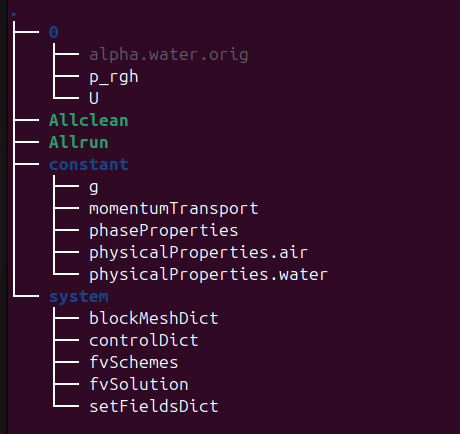
\includegraphics[width=0.5\linewidth]{tree-dambreak.png}
  \caption{Archivos de \texttt{damBreakLaminar}}
\end{figure}

El primer archivo que vamos a editar es \texttt{system/blockMeshDict}. En este archivo se definen tres partes: \texttt{vertices}, \texttt{blocks} y \texttt{boundary}.

\begin{itemize}
  \item En \texttt{vertices} colocamos todos los vértices de las caras de nuestro \textit{mesh} con el formato $(x\;y\;z)$. Al terminar de colocar los puntos, estos quedarán enlistados comenzando por el 0 según su aparición en el código.
  \item En \texttt{blocks} definimos los bloques mediante los puntos. La sintaxis es: 
  \begin{verbatim}
    hex (p1 p2 p3 ... p8) (a b c)
  \end{verbatim}
  Los 8 puntos deben colocarse de manera que si existe una arista entre dos puntos, estos aparezcan consecutivos en la lista. Los valores $a$, $b$ y $c$ indican la división del bloque en cada dirección.
  \item En \texttt{boundary} definimos las paredes de los bloques. Los tipos más comunes son:
  \begin{itemize}
    \item \texttt{type wall}: pared sólida dentro del dominio.
    \item \texttt{type patch}: permite entrada y salida de fluido; no aporta información sobre la pared.
    \item \texttt{type symmetryPlane}: replica lo que ocurre en el plano de simetría.
    \item \texttt{type empty}: útil para modelar en 2D o 1D, ya que el sistema no resuelve ecuaciones en esas direcciones.
  \end{itemize}
\end{itemize}

Al determinar las paredes, podemos agrupar distintas caras si tienen el mismo tipo o alguna propiedad particular que será importante más adelante. A esto se le llama \texttt{boundaryField}.

Para verificar cómo quedó el \textit{mesh}, usamos los comandos:
\begin{verbatim}
blockMesh
paraFoam
\end{verbatim}
\texttt{blockMesh} compila el código y \texttt{paraFoam} abre un visualizador para ver el \textit{mesh}.

\begin{figure}[h]
  \centering
  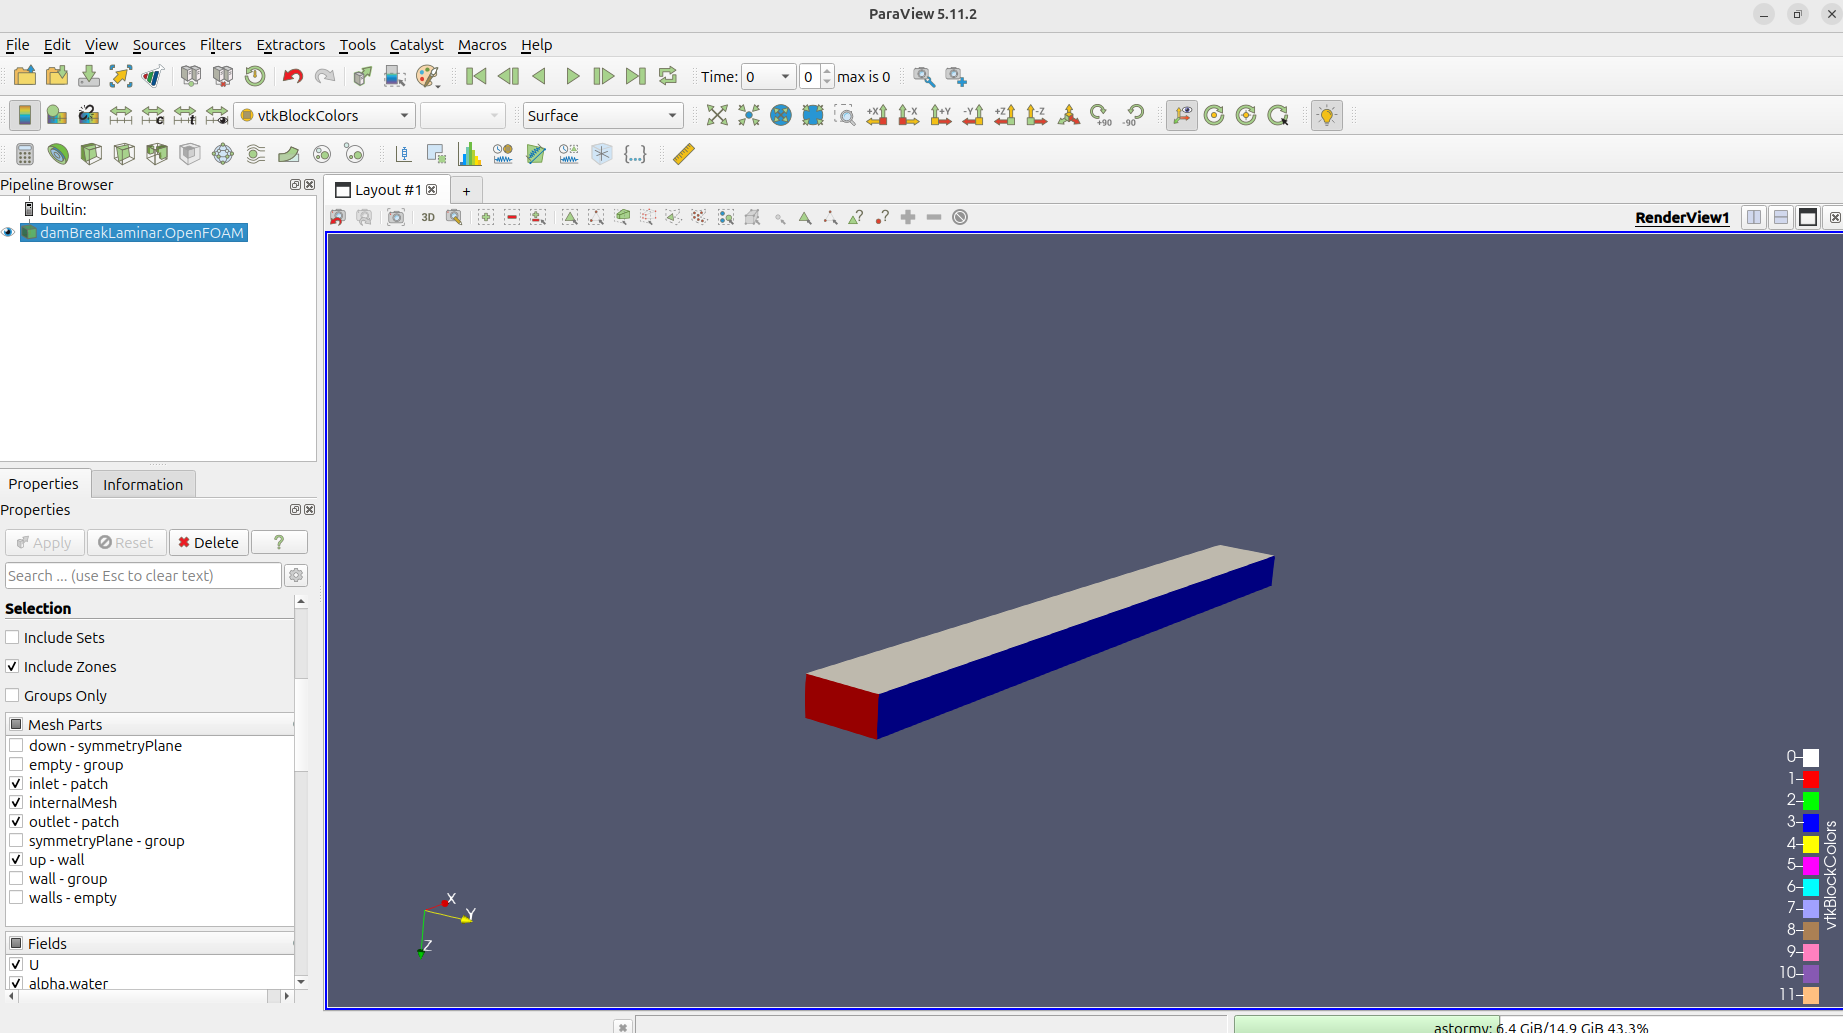
\includegraphics[width=0.9\linewidth]{modelo_3d.png}
  \caption{Modelo 3D del dominio}
\end{figure}

Ahora editaremos las condiciones iniciales del sistema, que se encuentran en la carpeta \texttt{0}. Empecemos con el archivo \texttt{U}, que contiene las velocidades del agua en las caras del sistema (llamado \texttt{boundaryMesh}). Los tipos que se pueden asignar son:

\begin{itemize}
  \item \texttt{fixedValue}: se asigna un valor fijo de velocidad mediante la línea \texttt{value uniform (vx vy vz)}.
  \item \texttt{zeroGradient}: la velocidad se obtiene de la celda vecina; se usa usualmente en las caras de salida.
  \item \texttt{symmetryPlane}: replica lo que ocurre en el plano de simetría.
  \item \texttt{noSlip}: produce paredes sin deslizamiento.
  \item \texttt{slip}: permite que el fluido resbale sobre la cara seleccionada.
  \item \texttt{empty}: no agrega ninguna condición.
\end{itemize}

También en la carpeta \texttt{0} tenemos el archivo \texttt{p\_rgh}, que representa la presión hidrostática. Aquí podemos modificar los tipos de \texttt{boundaryField}. Los tipos son los mismos que en \texttt{U}, excepto \texttt{slip} y \texttt{noSlip}. Se añade además \texttt{fixedFluxPressure}, que es una presión fija determinada por el sistema.

Con esto solo quedaría revisar las propiedades físicas del aire y del agua. Estos archivos están en la carpeta \texttt{constant}. Podemos modificar la viscosidad (\texttt{nu}) y densidad (\texttt{rho}) del líquido y del aire en los archivos \texttt{physicalProperties.water} y \texttt{physicalProperties.air}, respectivamente. También debemos modificar \texttt{phaseProperties}, donde definimos las fases del líquido con \texttt{phases (water air)} y el coeficiente de tensión superficial (\texttt{sigma}).

Los siguientes archivos que agreguemos o modifiquemos estarán relacionados con si el flujo es laminar o turbulento.

\subsection{Flujo laminar}

Para flujo laminar, como el ejemplo que estamos usando ya emplea este modelo, solo mostraremos dónde se define. Abrimos la carpeta \texttt{constant} y el archivo \texttt{momentumTransport}. Allí podemos ver la variable \texttt{simulationType} con el valor \texttt{laminar}.

\subsection{Flujo turbulento}

Para flujo turbulento, debemos modificar el archivo \texttt{constant/momentumTransport} y establecer \texttt{simulationType RAS} (Reynolds-Averaged Simulation). Debajo de esto indicamos que usaremos el modelo \texttt{kEpsilon} y que hay turbulencia.

\begin{figure}[h]
  \centering
  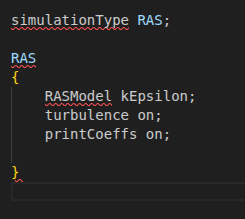
\includegraphics[width=0.3\linewidth]{ras_file.png}
  \caption{Formato del archivo \texttt{RAS}}
\end{figure}

Además, debemos agregar los siguientes archivos en la carpeta \texttt{0}: \texttt{k}, \texttt{nut} y \texttt{epsilon}. Empecemos con \texttt{k}, donde se define la energía cinética turbulenta. En este archivo debemos especificar los \texttt{boundaryField}. Las opciones principales son:

\begin{itemize}
  \item \texttt{fixedValue}: se asigna un valor fijo.
  \item \texttt{inletOutlet}: se usa cuando la dirección del flujo es desconocida.
  \item \texttt{symmetryPlane}
  \item \texttt{zeroGradient}
  \item \texttt{empty}
\end{itemize}

Luego revisamos \texttt{epsilon}, que representa la tasa de disipación de la energía cinética turbulenta, y tiene los mismos tipos que \texttt{k}. Finalmente, \texttt{nut} es la viscosidad turbulenta.

\subsection{Agregar funciones de medición}

En el archivo \texttt{system/controlDict}, al final podemos agregar funciones de medición mediante la definición de \texttt{functions} y \texttt{probes} de la siguiente manera:

\begin{figure}[h]
  \centering
  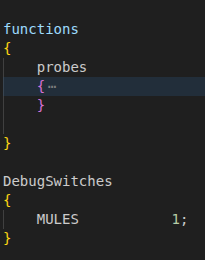
\includegraphics[width=0.4\linewidth]{funciones.png}
  \caption{Ejemplo de funciones de medición en \texttt{controlDict}}
\end{figure}

Dentro de \texttt{probes}, si queremos medir la presión, hacemos lo siguiente: primero definimos el campo que nos interesa (en este caso la presión, que está en el archivo \texttt{p\_rgh}) y luego indicamos los puntos donde queremos medir mediante \texttt{probeLocations}.

\begin{figure}[h]
  \centering
  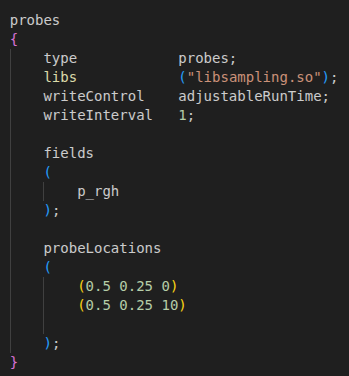
\includegraphics[width=0.4\linewidth]{probes_function.png}
  \caption{Función de medición de presión con \texttt{probes}}
\end{figure}

\subsection{Ejecución del programa}

Para ejecutar el programa usamos:
\begin{verbatim}
foamRun
\end{verbatim}
Para visualizar los resultados:
\begin{verbatim}
paraFoam
\end{verbatim}
Una vez dentro de ParaView, cambiamos \texttt{Solid Color} por \texttt{alpha.water} y obtenemos una visualización similar a la siguiente:

\begin{figure}[h]
  \centering
  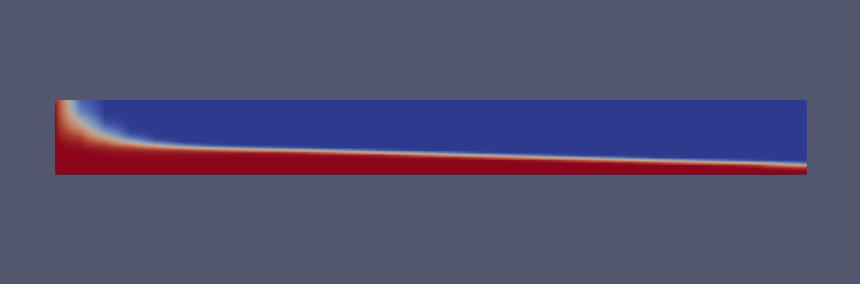
\includegraphics[width=0.6\linewidth]{fluido_mov1.png}
  \caption{Movimiento del fluido (campo \texttt{alpha.water})}
\end{figure}

\end{document}
